\documentclass{article}

\usepackage[english]{babel}
\usepackage[utf8]{inputenc}
\usepackage{cleveref}
\usepackage{tikz}

\usetikzlibrary{automata,arrows,positioning}

\begin{document}
\begin{figure}
\centering
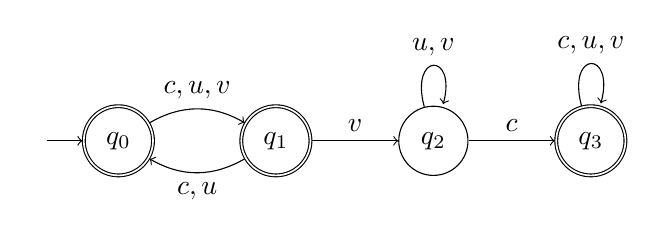
\begin{tikzpicture}[auto,node distance=2cm]
\node[state,initial,accepting,initial text={}] (q0) {$q_0$};
\node[state,accepting] (q1)[right of=q0] {$q_1$};
\node[state] (q2)[right of=q1] {$q_2$};
\node[state,accepting] (q3)[right of=q2] {$q_3$};

\path[->]	(q0) edge[bend left] node {$c, u, v$} (q1)
			(q1) edge[bend left] node {$c, u$} (q0)
			(q1) edge node {$v$} (q2)
			(q2) edge[loop above] node {$u, v$} (q2)
			(q2) edge node {$c$} (q3)
			(q3) edge[loop above] node {$c, u, v$} (q3)
;;
\end{tikzpicture}
\caption{Property showing that we were not optimal}
\label{fig:propOptimality}
\end{figure}

In \cref{fig:propOptimality}, we can see that using only $Q_{\mathrm{enf}}$ is 
not optimal, because when $c . c$ is received, it is possible to emit $c$, which 
would not be done using only $Q_{\mathrm{enf}}$. It is possible to emit $c$ 
because in this property, all that is necessary is to avoid state $q_2$, which 
is possible if there is at least one $c$ in the buffer. Thus, when $c . c$ is 
received, the first one can be emitted. This property is defined in the file 
\textsf{prop1.tmtn}, that can be given to the \textsf{test} executable, that 
will then enforce it.

\end{document}

